\documentclass{ximera}

\newcommand{\RR}{\mathbb R}
\renewcommand{\d}{\,d}
\newcommand{\dd}[2][]{\frac{d #1}{d #2}}
\renewcommand{\l}{\ell}
\newcommand{\ddx}{\frac{d}{dx}}
\newcommand{\dfn}{\textbf}
\newcommand{\eval}[1]{\bigg[ #1 \bigg]}


\outcome{Relate the graph of a function to the graph of its derivative.}

\author{Nela Lakos \and Kyle Parsons}

\begin{document}
\begin{exercise}

The figure below shows the graphs of $f$, $f'$ and another function $g$.  Which curve is which?


\begin{image}
  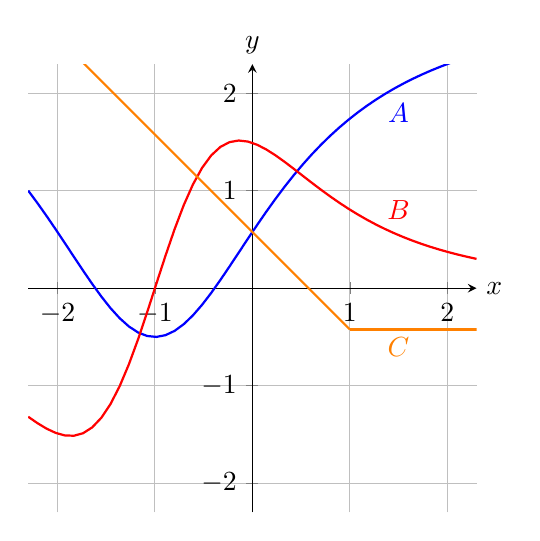
\begin{tikzpicture}
    \begin{axis}[
        xmin=-2.3,xmax=2.3,ymin=-2.3,ymax=2.3,
        clip=true,
        unit vector ratio*=1 1 1,
        axis lines=center,
        grid = major,
        ytick={-2,-1,...,2},
    xtick={-2,-1,...,2},
        xlabel=$x$, ylabel=$y$,
        every axis y label/.style={at=(current axis.above origin),anchor=south},
        every axis x label/.style={at=(current axis.right of origin),anchor=west},
      ]
      \addplot[thick,blue,domain=-2.3:2.3,samples=50] plot{-3.5/(1+((x+1)/1.5)^2) + 3};
      \node at (axis cs:1.5,1.8) [blue] {$A$};
      
      \addplot[thick,red,domain=-2.3:2.3,samples=50] plot{14/3*((x+1)/1.5)/(1+((x+1)/1.5)^2)^2};
      \node at (axis cs:1.5,0.8) [red] {$B$};
      
      \addplot[thick,orange,domain=-2.3:1] plot{15/26-x};
      \addplot[thick,orange,domain=1:2.3] plot{-11/26};
      \node at (axis cs:1.5,-0.6) [orange] {$C$};

      \end{axis}`
  \end{tikzpicture}
\end{image}

Input the correct curve for each function.
\begin{align*}
f &= \answer{A}\\
f' &= \answer{B}\\
g &= \answer{C}
\end{align*}

\end{exercise}
\end{document}